\documentclass{university}

\course{هوش مصنوعی}
\subject{آزمون میانترم}
\professor{دکتر رهبان}

\begin{document}

\setupdocument

\section{سوالات کوتاه پاسخ}
\subsection{}
\subsubsection{}
درست، چون الگوریتم 
\lr{A*} 
یک الگوریتم سرچ 
\lr{informed} 
است، و تابع هیوریستیک 
\lr{monotonic} 
و در نتیجه 
\lr{admissible} 
است، این الگوریتم نودهای کمتری را 
\lr{expand} 
می‌کند تا به جواب برسد. 

\subsubsection{}
درست، اگر در الگوریتم اول بهترین تابع 
\lr{$f(n)$} 
سطر مربوط به نود باشد، جستجو به جستجو عمق اول تبدیل می‌شود.

\subsubsection{}
غلط، زمان اجرا الگوریتم 
\lr{beam search}
بستگی به عمق رفته شده دارد.

\subsection{}
\subsubsection{}
در حالت عادی حداکثر به تعداد برگ‌ها منهای یک باید 
\lr{backtracking}
انجام شود که این مقدار 
\lr{$d^n - 1$}
است. در صورت استفاده از الگوریتم‌های گفته شده باز هم 
\lr{worst case} 
تغییری نمی‌کند.

\subsubsection{}
\lr{$O(e \times d^2)$} 
که در آن 
\lr{$e$}
تعداد یال‌ها می‌باشد و 
\lr{d} 
اندازه دامنه است. 


\section{سوالات تشریحی}
\subsection{}
\subsubsection{}
\lr{$m$} 
عددی بزرگتر از یک است. 
\lr{$n$} 
نیز عددی بزرگتر از یک است. موقعیت هر 
\lr{agent} 
نیز 
\lr{$m$} 
حالت دارد که با توجه به نقشه بازی 
\lr{$(x, y)$}
مشخص می‌شود.

\subsubsection{}
اندازه فضای حالت توصیف شده، با توجه به اینکه هر 
\lr{pacman} 
به تعداد 
\lr{$m$}
موقعیت دارد و 
\lr{$n$} 
پکمن داریم، 
\lr{$m^n$}
است. 

\subsubsection{}
از آنجایی که هر 
\lr{pacman}
در هر مرحله 5 حرکت دارد، و 
\lr{$n$}
پکمن داریم، کران بالای 
\lr{branching factor} 
برابر 
\lr{$5^n - 1$}
است. چون ممکن است با توجه به موقعیت یک سری حرکات غیر مجاز باشند(مثلا سمت راست پکمن خالی در نقشه نباشد) 
و در صورتی که هیچ 
\lr{agent}ی
حرکت نکند به استیت جدید نمی‌رویم،
تعداد یال‌ها همیشه از عدد گفته شده کمتر است. 

\subsubsection{}
چون 
\lr{UCS} 
یک نوع سرچ 
\lr{uninformed} 
است، در همه جهات جستجو انجام می‌دهد. همچنین جستجو در عمق بیشترین فاصله منهتنی دو پکمن به 
جواب بهینه می‌رسد. چون جواب بر حسب 
\lr{$m$} و \lr{$n$} 
خواسته شده، ابتدا کران بالایی برای بیشترین فاصله منهتنی دو پکمن پیدا می‌کنیم سپس این عدد که کرانی برای عمق هست را 
استفاده می‌کنیم. 

چون 
\lr{$m$} 
خانه داریم، حداکثر فاصله دو پکمن وقتی است که این خانه‌ها به صورت خطی باشند و دو پکمن در 
ابتدا و انتهای آن باشند که در این صورت فاصله آن‌ها 
\lr{$\frac{m}{2}$}
است. دقت شود که هر دو حرکت می‌کنند و فاصله برای همین تقسیم صحیح بر 2 شده است. 

حال با اطلاعات موجود کران گره‌های بسط داده شده را بدست می‌آوریم. 
\begin{gather*}
    bound = 1 + b + b^2 + b^3 + ... + b^{depth-1} = \frac{b^{depth} - 1}{b - 1}\\
    b = 5^n - 1 \\
    depth = \frac{m}{2} \\
    \Rightarrow bound = \frac{(5^n-1)^{\frac{m}{2}}}{5^n - 2}
\end{gather*}

\subsubsection{}
اگر دو دورترین 
\lr{agent}ها 
را در نظر بگیریم، برای قرارگیری این دو در یک خانه، باید هر کدام حداقل به اندازه نصف فاصله منهتنی‌شان به سمت 
یکدیگر حرکت کنند. از آنجای که فاصله منهتنی جمع مولفه‌ها است و در این تابع بین مولفه‌ها ماکس گرفته شده، 
پس این تابع از تابع من کوچکتر است(تابع من تابع گفته شده را دامیننت می‌کند). در نتیجه 
تابع گفته شده 
\lr{admissible} 
است. 

حال اگر دو دورترین
\lr{agent} 
حرکت نکنند، نا مساوری مثلثی برقرار است چون تابع هیوریستیک تغییر نمی‌کند (یا بیشتر می‌شود با توجه به حرکت بقیه) و 
\lr{cost} 
بزرگتر از صفر است. از طرف دیگر اگر موقعیت دو دورترین تغییر کند و از هم دور شود باز هم نامساوی 
مثلثی بدون مشکل برقرار است چون تابع هیوریستیک ما بیشتر می‌شود. 
در صورتی که دو دورترین 
\lr{agent} 
به هم نزدیک شوند، تابع هیوریستیک حداکثر 
\lr{$\frac{1}{2} \times 1$}
واحد کاهش میابد که در این صورت 
\lr{cost} 
حرکت آن را جبران می‌کند. پس در همه حالات نامساوی مثلثی برقرار است و 
تابع هیوریستیک داده شده 
\lr{monotonic} 
است. 

\subsection{}
\subsubsection{}
\begin{gather*}
    \text{تابع $g(x)$ محدب است} \Rightarrow \frac{d^2 f(x)}{d x^2} > 0 \\
    \text{تابع $f(x)$ محدب است} \Rightarrow \frac{d^2 g(x)}{d x^2} > 0 \\
    h(x) = f(x) + g(x) \\
    \text{مشتق عملگر خطی است} \Rightarrow \frac{d^2 h(x)}{d x^2} = \underbrace{\frac{d^2 f(x)}{d x^2}}_{\text{مثبت}} + \underbrace{\frac{d^2 g(x)}{d x^2}}_{\text{مثبت}} \\
    \Rightarrow \frac{d^2 h(x)}{d x^2} > 0 \Rightarrow \text{تابع $h(x)$ نیز محدب است}
\end{gather*}

\subsubsection{}
\begin{gather*}
    \text{تابع $g(x)$ محدب است} \Rightarrow \forall x,y \in \mathbb{R}, 0 \leq \theta \leq 1 :
    f(\theta x + (1-\theta) y) \leq \theta f(x) + (1 - \theta) f(y)\\
    \text{تابع $f(x)$ محدب است} \Rightarrow \forall x,y \in \mathbb{R}, 0 \leq \theta \leq 1 :
    g(\theta x + (1-\theta) y) \leq \theta g(x) + (1 - \theta) g(y)\\
    h(x) = max\{f(x), g(x)\} \\ 
    \Rightarrow \forall x,y \in \mathbb{R}, 0 \leq \theta \leq 1 : \\
    h(\theta x + (1-\theta) y) = max\{f(\theta x + (1-\theta) y), g(\theta x + (1-\theta) y)\} \\
    \theta h(x) = max\{\theta f(x), \theta g(x)\} 
    \Rightarrow \theta h(x) \geq \theta f(x), \theta g(x) \\
    (1 - \theta) h(y) = max\{(1 - \theta) f(y), (1 - \theta) g(y)\} \\
    \Rightarrow (1 - \theta) h(y) \geq (1 - \theta) f(y), (1 - \theta) g(y) \\
    \Rightarrow
    \begin{cases}
        \theta h(x) + (1 - \theta) h(y) \geq \theta f(x) + (1 - \theta) f(y) \\
        \theta h(x) + (1 - \theta) h(y) \geq \theta g(x) + (1 - \theta) g(y) \\
        \theta h(x) + (1 - \theta) h(y) \geq \theta f(x) + (1 - \theta) g(y) \\
        \theta h(x) + (1 - \theta) h(y) \geq \theta g(x) + (1 - \theta) f(y)
    \end{cases} \\
    \Rightarrow h(x) + (1 - \theta) h(y) \geq max\{f(\theta x + (1-\theta) y), g(\theta x + (1-\theta) y)\} \\
    \Rightarrow h(x) + (1 - \theta) h(y) \geq h(\theta x + (1-\theta) y) 
    \Rightarrow \text{تابع $h(x)$ نیز محدب است}
\end{gather*}

\subsection{}
در این 
\lr{CSP} 
چهار متغیر وجود دارد که دامنه هر کدام در ابتدا اعداد 1 تا 3 می‌باشد. همچنین قیود نیز مشخص است. 

\subsubsection{}
گراف قیود در شکل 
\ref{fig:31}
آمده است.
\begin{figure}
    \centering
    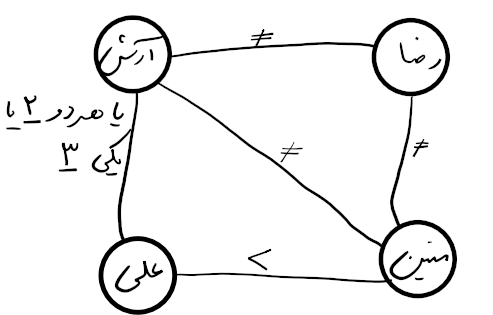
\includegraphics[width=\textwidth]{assets/3-1.png}
    \caption{گراف قیود}
    \label{fig:31}
\end{figure}

\subsubsection{}
اگر یال بین هر دو فرد را با شماره مشخص کنیم، مراحل شکل طی 
\ref{fig:32}
می‌شود. 

\begin{figure}
    \centering
    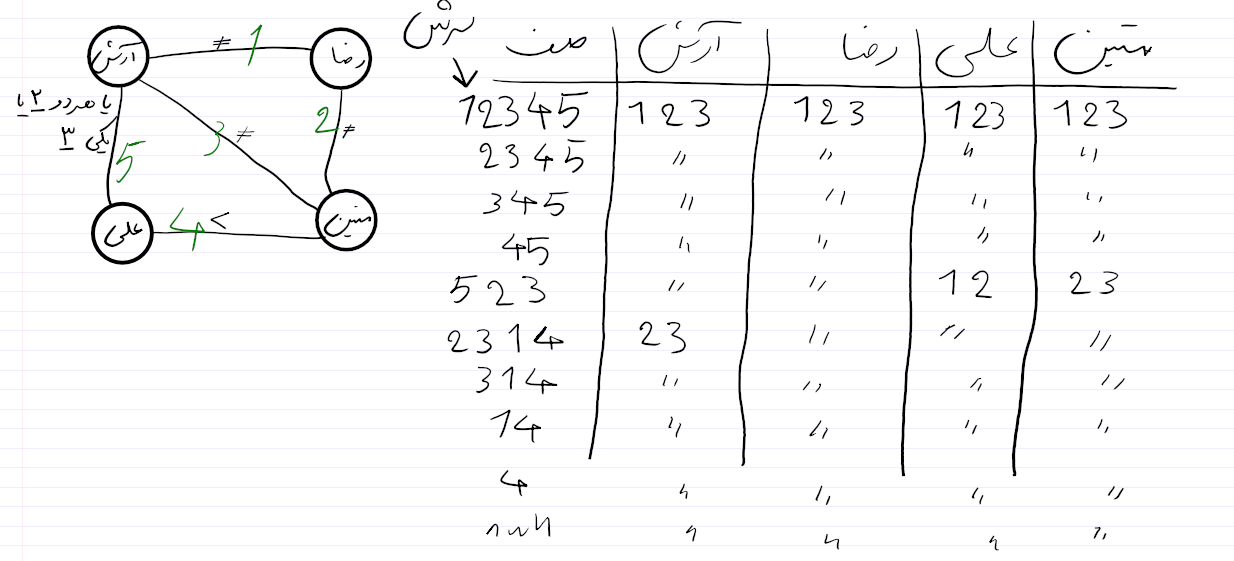
\includegraphics[width=\textwidth]{assets/3-2.png}
    \caption{کانسیستنت کردن}
    \label{fig:32}
\end{figure}

 \begin{itemize}
     \item علی: 1 2
     \item رضا: 1 2 3
     \item آرش: 2 3
     \item متین: 2 3
 \end{itemize}

\subsubsection{}
یال بین آرش و متین نقض می‌شود. 
با توجه به الگوریتم 
\lr{MRV} 
برای انتخاب متغیر آرش و علی و متین کمترین مقادیر باقیمانده را دارند(هر کدام یک مقدار باقیمانده دارند).
چون در اینجا 
\lr{tie} 
شده‌اند، آرش انتخاب می‌شود چون از نظر الفبایی از بقیه جلوتر است. با توجه به 
\lr{min conflict value} 
مقدار 2 برای آن انتخاب می‌شود که هر دو قید نقض شده را ارضا می‌کند. 

\subsection{}
\subsubsection{}
مقدار ریشه 2 است که در شکل 
\ref{fig:41}
نمایش داده شده است.
\begin{figure}
    \centering
    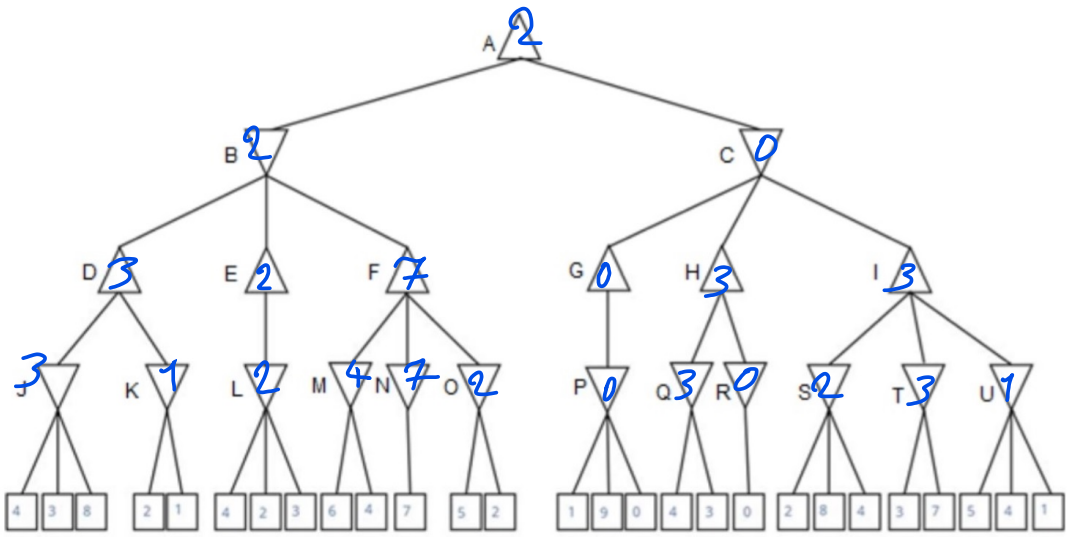
\includegraphics[width=\textwidth]{assets/4-1.png}
    \caption{مقدار ریشه}
    \label{fig:41}
\end{figure}

\subsubsection{}
شاخه‌های هرس شده در شکل 
\ref{fig:42}
نمایش داده شده است.
\begin{figure}
    \centering
    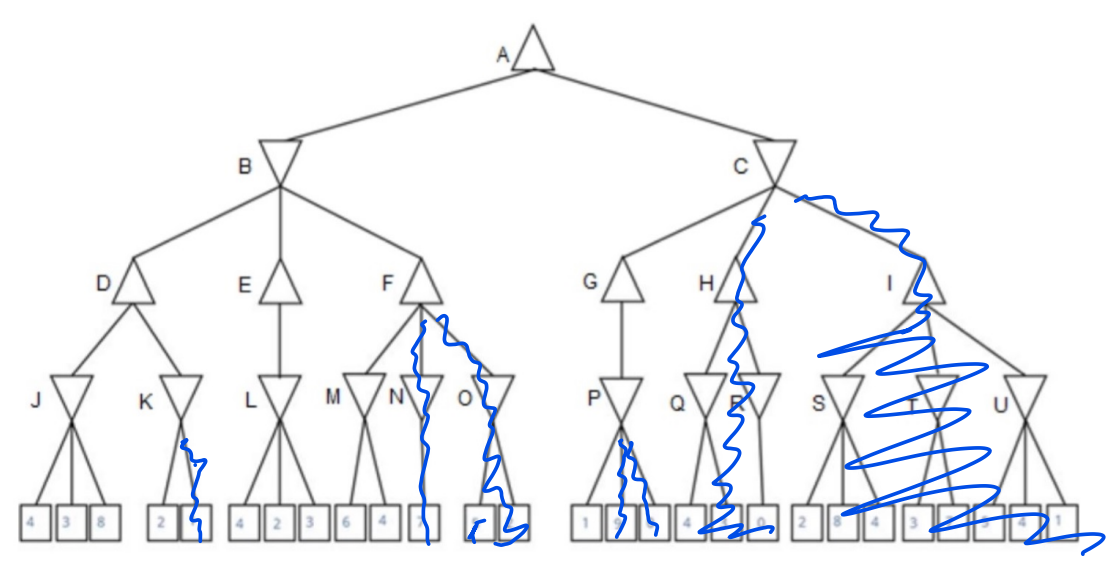
\includegraphics[width=\textwidth]{assets/4-2.png}
    \caption{شاخه‌های هرس شده}
    \label{fig:42}
\end{figure}

\end{document}